\documentclass[output=paper,colorlinks,citecolor=brown]{langscibook}
\ChapterDOI{10.5281/zenodo.15006607}
\author{Janine Siewert\orcid{}\affiliation{University of Helsinki} and
        Yves Scherrer\orcid{}\affiliation{University of Helsinki; University of Oslo} and
        Martijn Wieling\orcid{}\affiliation{University of Groningen}}
\title{Corpus-based Low Saxon dialectometry}

\abstract{In this corpus-based study, we explore how the similarity of Low Saxon dialects among each other and to the state languages Dutch and German has changed from the 19\textsuperscript{th} century to today. In particular, we want to investigate if the traditional classification into an eastern and a western group is visible in the data and if the Low Saxon dialects can be found to diverge at the Dutch-German border.

We apply principal component analysis and hierarchical clustering to n-grams of characters, part of speech tags and morphological features and observe divergent developments at the separate levels. As a reflection of different orthographic traditions, a noticeable distance between Dutch Low Saxon and German Low Saxon can be attested at the character level. At the PoS and morphological level, we however find a particular closeness between Dutch Low Saxon and the northern dialects from Germany, while we see German Westphalian in an outlier position. A shift towards the state languages can be observed at the PoS level, but the overall distance between Dutch Low Saxon and German Low Saxon does not seem to markedly increase at the three levels we studied.}

\IfFileExists{../localcommands.tex}{
   \addbibresource{../localbibliography.bib}
   \usepackage{tabularx,multicol}
%\usepackage{multirow}
\usepackage{subcaption}
\usepackage{url}
\urlstyle{same}

\usepackage{datetime}
\usepackage{enumitem}
\usepackage{langsci-optional}
\usepackage{langsci-lgr}
\usepackage{langsci-branding}

\usepackage{longtable}
\usepackage{xltabular}
\usepackage[linguistics, edges]{forest}
\usepackage{pgfplots}
\pgfplotsset{compat=1.18}
\usetikzlibrary{patterns, tikzmark}
\usepackage{pgfplotstable}
\usepgfplotslibrary{colorbrewer}
\usepackage{listings}
\lstset{basicstyle=\ttfamily,keywordstyle=\normalfont,language=,breaklines=true}

\usepackage{siunitx}
\sisetup{group-digits=none, detect-all=true}

\usepackage{langsci-gb4e}

   \makeatletter
\let\thetitle\@title
\let\theauthor\@author
\makeatother

% Use this Chinese font shipped with TeX Live instead of Source Han, because
% it is more portable/leightweight. Install the "fandol" package from CTAN to
% automatically get this font.
\newfontfamily{\ChineseFandolSong}{FandolSong-Regular.otf}

   %% hyphenation points for line breaks
%% Normally, automatic hyphenation in LaTeX is very good
%% If a word is mis-hyphenated, add it to this file
%%
%% add information to TeX file before \begin{document} with:
%% %% hyphenation points for line breaks
%% Normally, automatic hyphenation in LaTeX is very good
%% If a word is mis-hyphenated, add it to this file
%%
%% add information to TeX file before \begin{document} with:
%% %% hyphenation points for line breaks
%% Normally, automatic hyphenation in LaTeX is very good
%% If a word is mis-hyphenated, add it to this file
%%
%% add information to TeX file before \begin{document} with:
%% \include{localhyphenation}
\hyphenation{
    a-na-ly-sis
    ap-proach-es
    ar-che-o-log-i-cal
    Ar-khan-gelsk
    be-schrei-ben
    Buch-holtz
    Che-lya-binsk
    con-so-nant
    dia-lect
    dia-lect-ology
    Di-a-lekt-for-schung
    Dia-lekt-for-schung
    East-pha-lian
    För-der-ung
    Ge-mein-schaft-lich-keits-ent-wür-fe
    his-tor-i-cal
    Hok-kai-do
    ja-pa-nese
    Ja-pa-nese
    Ka-go-shi-ma
    Ka-li-nin-grad
    Knja-zev
    Ma-kro-be-reich
    Ma-lay-sia
    mor-pho-log-i-cal
    Mos-cow
    Nef-te-yu-gansk
    non-mobile
    nu-cle-ar
    ös-ter-rei-chi-sche
    par-a-digm
    per-zep-ti-ons-lin-gu-is-ti-sche
    plu-ri-zen-tri-schen
    quick-ly
    Reich
    Sax-on
    Schrö-der
    sear-ching
    ste-reo-type
    strength-en-ing
    strong-est
    Stutt-gart
    su-pra-seg-men-tal
    teach-er
    to-po-gra-phy
    To-ron-to
    tra-di-tion-al
    ul-ti-mate-ly
    Um-gangs-spra-che
    Volks-kun-de
    vor-zu-stel-len
    wheth-er
    Wie-sing-er
    with-in
    Wort-at-las
}

\hyphenation{
    a-na-ly-sis
    ap-proach-es
    ar-che-o-log-i-cal
    Ar-khan-gelsk
    be-schrei-ben
    Buch-holtz
    Che-lya-binsk
    con-so-nant
    dia-lect
    dia-lect-ology
    Di-a-lekt-for-schung
    Dia-lekt-for-schung
    East-pha-lian
    För-der-ung
    Ge-mein-schaft-lich-keits-ent-wür-fe
    his-tor-i-cal
    Hok-kai-do
    ja-pa-nese
    Ja-pa-nese
    Ka-go-shi-ma
    Ka-li-nin-grad
    Knja-zev
    Ma-kro-be-reich
    Ma-lay-sia
    mor-pho-log-i-cal
    Mos-cow
    Nef-te-yu-gansk
    non-mobile
    nu-cle-ar
    ös-ter-rei-chi-sche
    par-a-digm
    per-zep-ti-ons-lin-gu-is-ti-sche
    plu-ri-zen-tri-schen
    quick-ly
    Reich
    Sax-on
    Schrö-der
    sear-ching
    ste-reo-type
    strength-en-ing
    strong-est
    Stutt-gart
    su-pra-seg-men-tal
    teach-er
    to-po-gra-phy
    To-ron-to
    tra-di-tion-al
    ul-ti-mate-ly
    Um-gangs-spra-che
    Volks-kun-de
    vor-zu-stel-len
    wheth-er
    Wie-sing-er
    with-in
    Wort-at-las
}

\hyphenation{
    a-na-ly-sis
    ap-proach-es
    ar-che-o-log-i-cal
    Ar-khan-gelsk
    be-schrei-ben
    Buch-holtz
    Che-lya-binsk
    con-so-nant
    dia-lect
    dia-lect-ology
    Di-a-lekt-for-schung
    Dia-lekt-for-schung
    East-pha-lian
    För-der-ung
    Ge-mein-schaft-lich-keits-ent-wür-fe
    his-tor-i-cal
    Hok-kai-do
    ja-pa-nese
    Ja-pa-nese
    Ka-go-shi-ma
    Ka-li-nin-grad
    Knja-zev
    Ma-kro-be-reich
    Ma-lay-sia
    mor-pho-log-i-cal
    Mos-cow
    Nef-te-yu-gansk
    non-mobile
    nu-cle-ar
    ös-ter-rei-chi-sche
    par-a-digm
    per-zep-ti-ons-lin-gu-is-ti-sche
    plu-ri-zen-tri-schen
    quick-ly
    Reich
    Sax-on
    Schrö-der
    sear-ching
    ste-reo-type
    strength-en-ing
    strong-est
    Stutt-gart
    su-pra-seg-men-tal
    teach-er
    to-po-gra-phy
    To-ron-to
    tra-di-tion-al
    ul-ti-mate-ly
    Um-gangs-spra-che
    Volks-kun-de
    vor-zu-stel-len
    wheth-er
    Wie-sing-er
    with-in
    Wort-at-las
}

   \boolfalse{bookcompile}
%    \togglepaper[23]%%chapternumber
}{}

% #1: sorting key, #2: prefix for citation, #3: prefix for bibliography
\DeclareRobustCommand{\VAN}[3]{#3} % set up for citation

\begin{document}
\graphicspath{{figures/siewert}}
\maketitle
\label{chap:siewert}

\section{Introduction}
In the context of a research project on dialectal variation in Low Saxon\footnote{Also referred to as “Low German”.}, we investigate how the similarity of larger dialect areas has changed from the 19\textsuperscript{th} to the 21\textsuperscript{st} century. Our study is based on corpus data that we have collected earlier and covers both the Dutch and the German side of the Low Saxon language area. 

% [HS] Traditional dialect classifications, such as the ones presented by \citet{Schroeder2004},
\begin{sloppypar}
Traditional dialect classifications, such as the ones presented by \citet{Schroeder2004},
have large\hyp ly relied on the occurrence of certain phonological and morphological traits. In this study, we however take a corpus-based approach and zoom in on three levels of the language: orthographic, morphological, and syntactic. Among possible differences at these three levels, we particularly want to investigate how the corpus-based results relate to the more traditional classifications and to the language contact situation. Therefore, we are interested in 1) the traditional east-west division, and 2) what the effect of the Dutch-German border is on the development of Low Saxon in recent decades.
\end{sloppypar}

%In connection with a research project on diachronic and synchronic variation in Low Saxon, we investigate dialect similarity in 19\textsuperscript{th} to 21\textsuperscript{st} century Low Saxon based on data from Germany and the Netherlands. Traditionally, Low Saxon dialect classification has mostly been based on phonological and morphological traits, such as the ones presented by \citet{Schroeder2004}. In this study, however, we are focusing on the orthographic, morphological and syntactic side, and compare how these relate to each other and to the more traditional classifications. 


%As in the 19\textsuperscript{th} century, school education and majority language media played a smaller role in everyday life than today, 

%We hypothesize that the effect of language contact with Dutch and German is less visible in the morphology and syntax of 19\textsuperscript{th} century Low Saxon, even though the border might already be discernable at the orthographic level. Therefore, we will investigate how these results compare to more modern data from the 21\textsuperscript{st} century.
%stärker allgemeinen syntaxvergleich betonen, grenzeffekte nur ein element
 %Furthermore, we are not only interested in the border region but in the whole language area, ... how syntactic and mophosyntactic approaches ... with more traditional dialect classifications relying more strongly on phonology, morphology and the lexicon. \citep{Schroeder2004} 

\section{Low Saxon dialect classification and variation}

\begin{figure}
    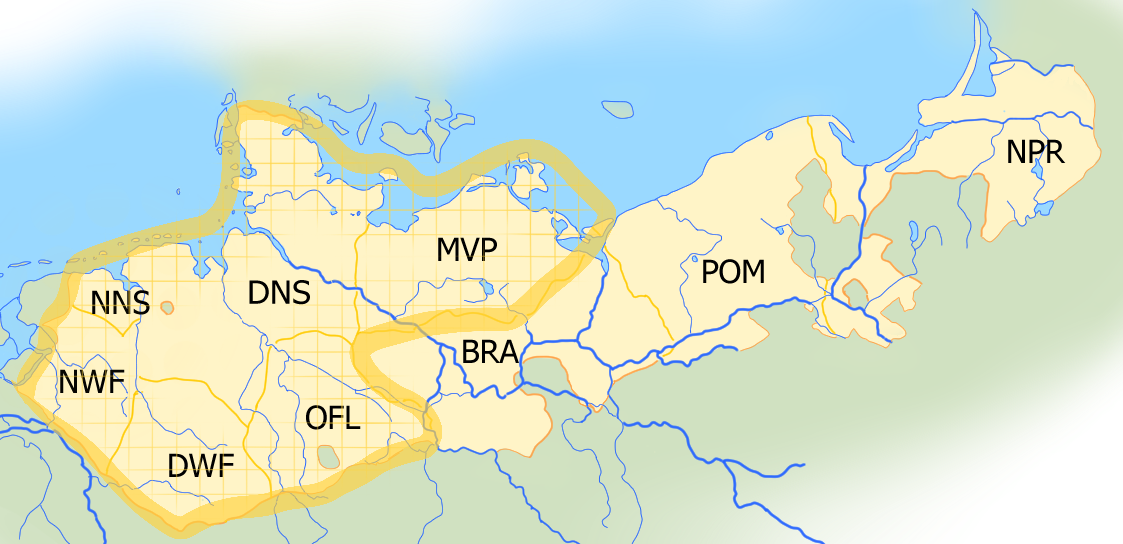
\includegraphics[width=\textwidth]{neddersassiske_dialekten_seminaar2022.png}
    \caption{Low Saxon dialects: NNS: Dutch North Saxon, NWF: Dutch Westphalian, DNS: German North Saxon, DWF: German Westphalian, MVP: Mecklenburgish--West Pomeranian, OFL: Eastphalian, BRA: Brandenburgish, POM: East Pomeranian, NPR: Low Prussian; self-created map}
    \label{fig:dialect_map}
\end{figure}

Low Saxon is a West-Germanic language primarily spoken in northern Germany and the north-eastern Netherlands. Despite official recognition in both countries, there is no common standard variety. As a result, Low Saxon speakers will typically speak and write their own dialect(s) in all language use contexts. 

\figref{fig:dialect_map} shows the Low Saxon language area in the early 20\textsuperscript{th} century with its major dialect groups. In this paper, we will focus on the encircled dialects. 

The dialect division of German Low Saxon follows the traditional classification presented by \citet{Schroeder2004} and \citet{Stellmacher1983}. This classification is primarily based on phonological and morphological traits such as vowel phoneme mergers and the plural ending of verbs in the present tense. Based on this plural suffix, \citet[240]{Stellmacher1983} divides German Low Saxon into an eastern and a western group, where \textit{-et} is used in the west and \textit{-en} in the east. Of the dialects included in our research, only Mecklenburgish-West Pomeranian (MVP) belongs to this eastern group.

A more fine-grained division is normally used for Dutch Low Saxon (see for instance \citealt[20]{BloemhoffEtAl2019}), possibly due to the much smaller size of the language area. In this cross-border comparison, we wanted to keep the size of the areas of comparison roughly in line with one another, but at the same time be able to look at internal differences within Dutch Low Saxon. As a compromise, we opted for a two-fold North-South division. Dutch North Saxon (NNS) is only represented by texts from Groningen in our dataset, while the southern part, called “Dutch Westphalian” (NWF) here, includes texts from Achterhoeks, Veluws, Twents, Sallands and Drents. This North-South division has a rough correspondence with German North Saxon (DNS) and German Westphalian (DWF).  

An important isogloss for dividing North Saxon from Westphalian is the merg\hyp er of Proto-Germanic *â and lengthened *a in the north contrasting with the preservation of distinct phonemes in the Westphalian dialects (\citealt{Niebaum2008}, \citealt{BloemhoffEtAl2019}). This distinction can still be found on both sides of the border.
In addition, the northern group of Dutch Low Saxon has a Frisian substrate which is likely why \citet{Jellinghaus1892}  refers to it as “Friso\hyp Saxon” and contrasts it with “Saxon” dialects. 

%Motivation for the north-south split in Dutch Low Saxon (cf. e-mail to Raoul):

%\textit{For this very rough and simplified split, I have mostly followed the isoglosses across the border since I am making cross-border comparisons. An important isogloss for dividing North Saxon from Westphalian on the German side is the merger of Proto-Germanic *â and lengthened *a in the north and the preservation of distinct phonemes in the south (mentioned also by \citet{Niebaum2008}). As far as I have observed, this distinction largely holds true for Northern vs. Southern Dutch Low Saxon as well, and this is also what \citet[35]{BloemhoffEtAl2019} say.
%The development of the old long vowels ē1-4, ō1-2 and ȫ1-2 in (most of) Groningen nicely connects to the adjacent North Saxon dialects on the German side, too. \citet{PanzerThuemmel1971} provide isogloss maps and tables with vowel realisations in many places from both the Dutch and the German side. I do not have the book to hand right now but could take a look tomorrow at the library, if necessary.
%At least in the older literature, there is a tradition of calling the southern part of Dutch Low Saxon “Dutch Westphalian” and putting Gronings into one subgroup with East-Frisian as “Friso-Saksisch”, or contrasting “Friso-Saxon” with “Saxon” dialects like \citet{Jellinghaus1892} did. The terminology might be a bit outdated nowadays as I cannot recall encountering it much in more modern literature, but the division appears to approximately correspond to the isoglosses mentioned above.}

%Traditional east-west division %Can I mention that this has felt unintuitive to me as a LS speaker or would this be too anecdotal?


\subsection{Orthographic differences}\label{orthography}
%Can I cite my own MA thesis here?

In addition to dialectal variation, we find a large variety of spelling traditions and personal writing habits. While regional language institutes or societies, publishers or individual language enthusiasts devise and spread their own spelling systems today, explicit normification was not this widespread in the 19\textsuperscript{th} century. Even today, every Low Saxon speaker does not adhere to the spelling that a local publisher from the same region might prefer. For instance, while textbooks from Mecklenburg--West Pomerania (MVP) (e.g., \citealt{Herrmann-Winter2006}) tend to use the spelling by Herrmann-Winter, and textbooks from several areas of German North Saxon (DNS) (e.g., \citealt{Arbatzat2016}, \citealt{HiestermannKonen-Witzel2021}) can often be seen to follow the SASS\footnote{Not an abbreviation but based on the family name of Johannes Saß.} spelling \citep{KahlThies2009}, some of the people who provided texts for our dataset had other spelling preferences. 

Local spelling traditions tend to draw inspiration from the majority language orthography to different degrees and in different ways. We will illustrate this with a few examples from our dataset. Sentence \REF{spelling_nwf} is from the Netherlands and sentences \REF{spelling_dns} and \REF{spelling_dwf} from Germany. This can easily be recognised by the capitalisation of nouns (e.g., \textit{Kaarten}, \textit{Ogen}, \textit{Dage}, \textit{Magister}) or lack thereof (\textit{leu}, \textit{weerde}, \textit{ding}). While not all Low Saxon writers from Germany capitalise nouns, it is a common trait. 


\ea\label{spelling_nwf} %%%\il{Dutch Westphalian}\is{spelling} %add "IPP" to subject index for this page %add "Low Saxon" to language index for this page
De leu veult gemènlik eerst de weerde van 'n ding, as ze 't nig hebt. \\
\glt `In general, people only become aware of the value of things when they do not have them.'\\
\ex\label{spelling_dns} %%% \is{spelling}\il{German North Saxon} %add "Low Saxon" to language index for this page
 %add "IPP" to subject index for this page
Arfest neem twe Kaarten to de eerst Klaß, un as ik daröver grote Ogen maak, lach he un meen, dat kunn darop staan, ik schull man instigen. \\
\glt `Arfest bought two first class tickets, and when I looked on at him with astonishment, he laughed and said that may be written there but I should just get on.'
\ex\label{spelling_dwf} %%% \is{spelling}\il{German Westphalian} %add "Low Saxon" to language index for this page %add "IPP" to subject index for this page
Eunige Dage später frogere de Magister, biu de veuer Johrestyien herren.\\
\glt `A few days later, the teacher asked what the four seasons were called.'
\z



Sentence \REF{spelling_nwf} furthermore shows two grapheme-phoneme correspondences typical for Low Saxon writing from the Netherlands: <eu> for /ø/ and <z> for /z/. In texts from Germany, one would rather expect <ö(ö)> and <s>. 


In Sentence \REF{spelling_dns} we find the letter <ß> for /s/,\footnote{Here used according to the old German orthography, where the <ß> replaced <ss> in coda position.} again a strong indicator of the text coming from Germany as this letter is likely not used in Dutch Low Saxon. In addition, we see a difference in the adaptation of German spelling rules between Sentence \REF{spelling_dns} and \REF{spelling_dwf}. In the word \textit{Johrestyien} `seasons' (compare German \textit{Jahreszeiten}) in \REF{spelling_dwf}, the <h> is used as part of a digraph marking a long vowel. According to some local spellings such as the SASS \citep{KahlThies2009}, the <h> should indeed be used as a length marker if it is written in the German cognate. However, such a principle is not followed by all Low Saxon writers in Germany as can be seen in Sentence \REF{spelling_dns}. If this writer had adhered to the same rule, we would find <nehm> `took' and <stahn> `stand' instead of <neem> and <staan>, compare \textit{nahm} and \textit{stehen} in German.


%This additional layer of variation probably explains why we have found it beneficial to train separate models for certain dialects even if these dialects did not differ strongly at, for instance, the Part of Speech (PoS) level. 



\subsection{Language contact}\label{language-contact}
Another layer of variation is added by the influence from the different state languages, Dutch and German. \citet{Goossens2019} indeed observed a replacement of certain local characteristics with features from the majority languages. He finds this to primarily affect the lexical level, but influence can by found at the phonological, morphological, and syntactic level as well. 

Influence on grammatical gender, a morphological feature relevant for our current research, is described by \citet[107--109]{BloemhoffEtAl2019}. Whereas in Dutch, masculine and feminine gender have merged to a common gender, there are Dutch Low Saxon dialects such as Twents, where this distinction has been preserved. \citet{BloemhoffEtAl2019} however find that speakers of Twents are increasingly unsure which of the two genders to assign to nouns with common gender in Dutch. 

In his comparison of two neighbouring dialects at the border, \citet{Smits2011} observes two different tendencies. While he finds more structural language loss, i.e., convergence towards the state language, on the Dutch side of the border, there is more overall language loss, i.e., language shift from Low Saxon to German, on the German side. Nevertheless, the remaining speakers on the German side retain more structural characteristics of their dialect than their neighbours from the Netherlands.

%One interesting area to pay attention to with respect to dialect distance is the Dutch-German border. Like Goossens (1997) observed, the Low Saxon dialects along the border have started to diverge under the influence of the majority languages. According to him, this divergence is most pronounced at the lexical level, but convergence towards the majority language has also been attested in phonology, morphology and syntax. While studies on the divergence of dialects along the border often focus on the occurrence and frequency of particular traits based on interviews, cf. \citet{Smits2011}, this study addresses the overall (dis)similarity in prose texts.



\subsection{Morphological and syntactic traits}
Next, we will discuss six %I might want to remove one of the features discussed as I have noticed that I cannot see it sufficiently well at the PoS level
morphological and syntactic traits where Low Saxon dialects differ from each other and/or from the respective majority language. We focus on the kind of structures that are visible at the PoS and morphological level and where we expect the majority languages to exert influence. %Can all these characteristics be captured by bi- and trigrams or could it be necessary to include 4-grams? 
The traits are presented in the same order in which we discuss them in \sectref{pos-level-results}, \sectref{posmorf-level-results} and \sectref{discussion}.

\subsubsection{Lack of the definite article}\label{feature:lack-of-definite-article}

According to \citet{Pheiff2022}, there are Low Saxon dialects where the usage of the definite article is less frequent than in Standard Dutch and German. He observes this to be particularly true for the north of Groningen but has attested the lack of a definite article in contexts where it would be obligatory in the majority languages in other regions as well. 

For instance, our dataset contains the following sentence in older German North Saxon (DNS): 

% % % \is{article} %add "IPP" to subject index for this page
%\ea
%\gll ai  zo'n   varkentien   in   huus   hebt\\
%if-you   such-a  piggy  in   house   have-\textsc{2sg/pl}\\
%\glt `if you have such a piggy in the house'
%\z
%\il{Low Saxon} %add "Low Saxon" to language index for this page]

%As de Bur'n Sett up Bedd wäsen weer
\ea
\gll As de Bur 'n Sett up Bedd wäsen weer.\\
when the  farmer a moment on  bed be.\textsc{past-ptcp} be.\textsc{pst.3sg}\\
\glt `When the farmer had been on the bed for a moment.'
\z
% % % \il{Low Saxon} %add "Low Saxon" to language index for this page

This sentence illustrates the tendency mentioned by \citet[147]{Pheiff2022} that the definite article is missing particularly after prepositions: While no article is used after \textit{up}, it does occur in \textit{de Bur} and \textit{'n Sett}. Proper nouns are another context where the usage of the definite article is less frequent. This is in line with the geographical distribution  of the definite article with proper nouns within German as well, where the use of the definite article with personal names decreases the further north you go \citep[150]{Pheiff2022}.

\subsubsection{Motion verb + (to/and) + infinitive}\label{to-infinitive}\label{feature:um-to}
German and Dutch combine motion verbs with the construction \textit{um zu}\slash\textit{om te} to express finality. In Low Saxon, while usage of \textit{üm to} is possible, plain \textit{to} similar to English occurs commonly as well:
% % % \is{motionverb} %add "IPP" to subject index for this page

\ea
\gll He    keem   na  de   Köök   to  fröhstücken. \\
     he          come.\textsc{pst}.\textsc{3sg}  to  the   kitchen  to   eat\_breakfast \\
\glt `He came to the kitchen to eat breakfast.' \citep[74]{Thies2010}
\z
% % % \il{Low Saxon} %add "Low Saxon" to language index for this page

In addition, in a few dialects, the infinitive can be connected with \textit{un/en} `and'. \citet[76]{Thies2010} mentions this construction for Schleswig and assumes Danish influence but, for instance, Wilhelm Wisser from Eastern Holstein uses it in his collection of fairy tales as well: %occurs in several fairytales, but their origin is not mentioned, possibly he also collected fairytales from outside (Eastern) Holstein? 
% % % \is{motionverb} %add "IPP" to subject index for this page

\ea
 \gll Hê    schall   mal    na ehr'n   Brôder M\d{a}n gahn un fragen den' mal. \\
     he      shall.\textsc{3sg}  once  to  her-\textsc{m}.\textsc{acc}   brother  moon  go    and   ask    that.\textsc{M}-\textsc{acc}   once \\
\glt `He should just go to her brother moon and ask him.' \citep[53]{Wisser1921}
\z
% % % \il{Low Saxon} %add "Low Saxon" to language index for this page

Furthermore, this construction is attested in Dutch Low Saxon dialects such as Stellingwerfs: \textit{Ie kun mar beter naor de zoolder \textbf{gaon en vang(en)} die moes} `You better go to the attic and catch the mouse.' \citep[191]{Bloemhoff2008a} %use of verb stem corresponds with North Frisian infinitive III as described by Temmo Bosse. How does this construction work in West Frisian? 
and Gronings: \textit{ik \textbf{goa hin en helpn} Kloas} `I will go and help Kloas.' \citep[114]{vanBree2008}.


\subsubsection{Case inflection}\label{feature:case}
Low Saxon dialects differ noticeably in how many cases nouns inflect for. In Medieval Low Saxon, we still find nominative, genitive, dative, and accusative \citep{Lasch1974}, but the modern varieties typically display a simplified case system. According to \citet[62]{Luecht2016}, East Frisian\footnote{Part of German North Saxon (DNS). Not to be confused with the East Frisian language Saterland Frisian.} does not inflect nouns for case. Usage of independent genitive forms is generally very restricted, but most German Low Saxon dialects still distinguish between nominative and accusative in singular masculine nouns, which can be seen in the form of the adjective and the article \citep[144, 191]{LindowEtAl1998}. 

Many German Low Saxon dialects have preserved remnants of the dative case that might be used in connection with certain prepositions. In the German North Saxon (DNS) Sentence \REF{dative_dns} from our dataset, after \textit{bi}, we see a form of the definite article resembling the masculine accusative. As the expected form in the accusative of this neuter noun would be \textit{'t}, this can be interpreted as a reduced version of the older dative form \textit{'m}.
% % % \is{dative} %add "IPP" to subject index for this page

\ea\label{dative_dns}
\gll Mi   weer   de   Sunn   to   grall   bi   'n   Läsen. \\
me    was    the    sun   too    bright    at    the.\textsc{dat}.\textsc{sg}    reading. \\
\glt `The sun was too bright for me while reading.'
\z
% % % \il{German North Saxon} %add "Low Saxon" to language index for this page



\textit{To} is another preposition where we often encounter the definite article of neuter nouns as \textit{'n} instead of otherwise expected \textit{'t}, e.g., in this German North Saxon (DNS) sentence from our dataset: \textit{Dat's to'n Lachen!} `That is ridiculous!' 

Independent productive dative forms have only been preserved in a few southern German Low Saxon dialects such as South Westphalian (part of DWF). While most northern dialects in Germany distinguish between \textit{de Disch} `the table' in the nominative and \textit{den Disch} in the non-nominative, parts of German Westphalia exhibit a three-fold distinction between \textit{de Disk}\footnote{The nominative form is not given by \citet[145]{LindowEtAl1998}, but based on the other forms they present, it likely looks like this.} in the nominative, \textit{dem Diske} in the dative, and \textit{den Disk} in the accusative \citep[144--145]{LindowEtAl1998}. 

Case distinctions are not commonly mentioned in descriptions of Dutch Low Saxon and neither have we encountered any in our data. Individual fossilised cases in fixed expressions similar to Dutch might however still exist. 
%Nominative-accusative distinction (at least in masculine nouns) in most of German Low Saxon %no case distinction in Dutch Low Saxon at all anymore, right? What about 19th century DLS? (nom-acc not relevant here as the lack of the distinction will not be visible in the annotation)

\subsubsection{Subjunctive}\label{feature:subjunctive}

Within German Low Saxon, there is a North-South divide in subjunctive usage. As can be seen in the i-mutated forms \textit{söl} and \textit{bekäme} in Sentence \REF{subjunctive-westphalian} from German Westphalia, a few southern Low Saxon dialects have preserved distinct subjunctive forms. 
% % % \is{subjunctive} %add "IPP" to subject index for this page

\ea\label{subjunctive-westphalian}
\gll Et   söl   mi    frögn,   wank   et   bekäme.\\
     it          shall.\textsc{pst}.\textsc{sbjv}.\textsc{3sg}  me    please  if-I   it get.\textsc{pst}.\textsc{sbjv}-\textsc{1sg}\\
\glt `I would be happy if I got it.'
\citep[299]{Saltveit1983} 
\z
% % % \il{Westphalian} %add "Low Saxon" to language index for this page

Productivity however decreases further north. In Sentence \REF{subjunctive-dns} from Schleswig-Holstein, we find no i-mutation in \textit{schusst} although \textit{irrealis} meaning can be deduced from the context. 
% % % \is{subjunctive} %add "IPP" to subject index for this page

\ea\label{subjunctive-dns}
\gll Du  schusst  man  lewer   to   Huus    gahn    hebben.\\
     you.\textsc{sg}      shall.\textsc{pst}-\textsc{2sg}    but    rather    to    house    go    have\\
\glt `You had better gone home.' \citep[300]{Saltveit1983}
\z
% % % \il{German North Saxon} %add "Low Saxon" to language index for this page

The past tense forms in many northern dialects in Germany may show i-mutation due to their origin in subjunctive forms, but synchronically, they have taken on the role of the past indicative and thus there is no formal difference between indicative and subjunctive. These indistinct forms in the northern dialects can function as both indicative and subjunctive \citep[298--301]{Saltveit1983}. 



In addition, \textit{irrealis} meaning can be expressed by means of auxiliary verbs such as \textit{willen} `to want', \textit{warden} `to become', \textit{schölen} `shall' and \textit{doon} `to do', (cf. \citealt{LindowEtAl1998}, who mainly describe German North Saxon (DNS)). %one or two example sentences? 
 %Or are there any traces? Given that the subjunctive has almost completely fallen out of use in Dutch, I would at least not expect much to be left and I don't think I have ever encountered anything subjunctive-like. 


We are not aware of the existence of distinct subjunctive forms in today's Dutch Low Saxon.

\subsubsection{Infinitivus pro participio (IPP)}\label{IPP}
\textit{Infinitivus pro participio} refers to the phenomenon in West-Germanic languages such as Dutch and German of using an infinitive instead of an expected past participle, for example: 
\ea
\gll Ich hätte das tun können.\\                
     I have\textsc{.pst.sbjv-1sg} that do\textsc{.inf} can\textsc{.inf}\\
\glt`I could have done that.' 
\z

\citet[1]{Schmid2005} lists “Low German”\footnote{Due to the name choice possibly only referring to varieties from Germany.} as one of the West Germanic languages where IPP-constructions do not appear, which is in line with \citet{LindowEtAl1998}. 
% % % \is{IPP} %add "IPP" to subject index for this page

\ea
\gll Korl                           hett      den      Text      nich    lesen   kunnt.\\
     Korl          has  the-\textsc{acc}.\textsc{sg}    text  not   read can.\textsc{pst}-\textsc{ptcp}\\
\glt`Korl could not read the text.' \citep[108]{LindowEtAl1998}
\z
% % % \il{Low Saxon} %add "Low Saxon" to language index for this page

\citet[66]{BloemhoffEtAl2019} present a more varied picture for Dutch Low Saxon. They state that the northern dialects Gronings and Stellingwerfs indeed do not know the IPP-construction, whereas, in the other Dutch Low Saxon dialects, they assume a correlation with presence or absence of the \textit{(g)e-}prefix in the past participle. 

The situation for German Low Saxon is also in fact more complex than presented above. Even in the north-western dialects on which the grammar by \citet{LindowEtAl1998} focuses, some speakers today do use the IPP-construction (personal observation), perhaps due to influence from Standard German. 


\subsubsection{Complementiser doubling in subordinate clauses}\label{feature:double-complementiser} %I don't think this is actually sufficiently well visible at the PoS level, might require the lemmata, so maybe better to remove from this paper and keep for a future one 
Similar to Frisian \citep[299]{Popkema2018}, but different from (Standard) German and Dutch, \textit{as} `as' or \textit{dat} `that' can occur as a second complementiser in subordinate clauses,  typically after question words.  This is well attested in Dutch Low Saxon, cf.~the following example from Gronings: 
% % % \is{as_dat} %add "IPP" to subject index for this page

\ea
 \gll  Ik    mout    waitn   wel   dat   ik   in   hoes   krieg. \\
     I      must.\textsc{1sg}  know  who  that    I    in   house   get.\textsc{1sg}\\
\glt `I need to know whom I will get into the house.' \citep[114]{vanBree2008}
\z
% % % \il{Low Saxon} %add "Low Saxon" to language index for this page

%Drents: \textit{hij wus niet meer \textbf{hoe as}-e d'r mit an mus} \citep[114]{vanBree2008}

%\textit{dat as} mentioned in \citet[216]{bloemhoffkocksniebaum2008}

This phenomenon is not commonly described in grammars for German Low Saxon but \citet[289, 330]{Saltveit1983}  briefly mentions the usage of both \textit{dat} and \textit{as} and offers two example sentences.
%\textit{ik viel vetn, \textbf{vurim as} dun hest loten rupm} 
%\textit{Stekk en Finger in'e Ern un rink, \textbf{in wekk Lanne, dat}te bist}
Moreover, we have encountered several examples with \textit{as} in literary works such as \citet{Wisser1921} and \citet{Peters1986}.
% % % \is{as_dat} %add "IPP" to subject index for this page

\ea
 \gll  Un dạrmit secht de ol Mann em Beschêd, wodenni as he dat maken schall.\\
     and   therewith   says  the   old   man  him  information    how    as    he   that    make       shall.\textsc{3sg}\\
\glt `And with this, the old man tells him how he should do it.' \citep[29]{Wisser1921}
\z
% % \il{Low Saxon} %add "Low Saxon" to language index for this page


%, e.g., \textit{Un d\d{a}rmit secht de ol Mann em Beschêd, \textbf{wodenni as} he dat maken schall.} \citep[29]{Wisser1921}. 
%since I have become aware of this construction I have started to notice it in several works of GLS literature. Hard to believe that it has been overlooked? 
\citet{SchallertEtAl2018} have found attestations of the variant with \textit{dat} already in Medieval Low Saxon. Its usage is however not restricted to Low Saxon, but  they point out that this type of construction occurs throughout West-Germanic and even neighbouring Romance and Slavonic varieties, in particular in the Alpine region. 


\section{Dataset}

Our dataset is taken from the PoS-tagged and morphologically annotated version\footnote{Please see \url{https://universaldependencies.org/u/pos/index.html} and \url{https://universaldependencies.org/u/feat/index.html} for a description of the PoS tags and morphological features.} of the LSDC dataset LSDC-morph \citep{SiewertEtAl2022}. %, from relevant prose texts from \citet{LeopoldLeopold1882}\footnote{Digitised by dbnl: \url{https://dbnl.nl/tekst/leop008sche00_01/}.} and the \textit{Twentse Taalbank} \citep{vanderVliet2021}. 

\begin{sloppypar}
The overall dataset covers eight dialect regions from the 19\textsuperscript{th}, 20\textsuperscript{th} and 21\textsuperscript{st} century, but in this study, we focus on these six major Low Saxon dialect groups: Dutch North Saxon (NNS), German North Saxon (DNS), Dutch Westphalian (NWF), German Westphalian (DWF), Eastphalian (OFL) and Mecklenburgish-West Pom\hyp eranian (MVP). The reason for excluding the other eastern dialects Brandenburgish (BRA), East Pomerian (POM) and Low Prussian (NPR) is the relatively low amount of data.
\end{sloppypar}

%short summary of data collection and content
The older part of the dataset consists primarily of copyright-free material available online, mainly on Wikisource, \citet{LeopoldLeopold1882}\footnote{Digitised by dbnl: \url{https://dbnl.nl/tekst/leop008sche00_01/}.} and the \textit{Twentse Taalbank} \citep{vanderVliet2021}. On the other hand, the modern data for most dialects was personally provided by a variety of local authors. Common genres in the dataset are short stories and short novels, but various other genres such as speeches, religious texts, historical accounts, fairy tales and letters are included as well. For a more detailed description of the content and data collection for the LSDC dataset, please see \citet{SiewertEtAl2020}. 

We split the data into two time periods: 1800--1939 and 1980--today\footnote{In practice, this likely means roughly 2000--today, but we do not have the exact year of publication/writing of every text that local authors provided.}. This split is motivated by the language shift to the respective majority language, which in most regions occurred between the 1940s and 1980s. %some source for this? 
A practical reason possibly connected to the language shift is the lack of data from the intermediate period. Only from German Westphalian (DWF) we have one text that was marked as published during this period and three additional short texts that might have been published then based on the authors' life dates. Another practical explanation for the lack of data might be that texts from this period are often still copyright-protected and therefore not easily available in digitised format. 

We thus have an older period, when Low Saxon was still the dominant language of oral communication, and a newer period, when (a regional version of) Dutch or German has become the primary language in everyday life.


%Overall, our dataset consists of 34,460 sentences and 345,131 tokens from the 19\textsuperscript{th} century, and 44,740 sentences and 740,849 tokens from the 21\textsuperscript{st} century. We have converted these to CoNLL-U format and automatically PoS tagged. %adapt numbers, better as a table
%Our dataset covers seven dialect regions: , Mecklenburgish--West Pomeranian and Brandenburgish - South Marchian. The average amount of sentences is 1976.5, ranging from 185 in Brandenburgish - South Marchian to 4949 in Dutch Westphalian. 
%In this rough division, Dutch Westphalian includes all Dutch Low Saxon dialects except for Gronings. More fine-grained metadata on for instance the subdialect, the writer and their place of birth is provided if available. 
%For Eastphalian and Brandenburgish, we have obtained several hundred additional sentences, for German Westphalian several thousand ones from e.g., the LSDC dataset \citep{SiewertEtAl2020} and other resources. These, however, still require further preprocessing. If accepted, our dataset will be published in connection with the conference. 

Our Standard German (DEU) and Standard Dutch (NDL) datasets are taken from Universal Dependencies.\footnote{\url{https://universaldependencies.org}} 
For German, we used the UD\_German\_HDT treebank \citep{BorgesVoelkerEtAl2019} and, for Dutch, both the UD\_Dutch-Alpino and the UD\_Dutch-LassySmall treebanks \citep{BoumavanNoord2017}. We filtered the Dutch and German treebanks to remove duplicate sentences. 

 The overall size of our dataset is shown in \tabref{tab:datasetsize} and our updated version of LSDC-morph dataset is made available at \url{https://github.com/Helsinki-NLP/LSDC-morph/tree/main/methods2022}.

\begin{table}
 \begin{tabularx}{\textwidth}{Q rrrr}
  \lsptoprule
            & \multicolumn{2}{c}{1800--1939} & \multicolumn{2}{c}{1980--2022}\\\cmidrule(lr){2-3}\cmidrule(lr){4-5}
            & Sentences & Tokens & Sentences & Tokens \\
  \midrule
  Dutch North Saxon (NNS)  & 1,828 & 44,067 & 17,796 & 261,342\\
  Dutch Westphalian (NWF) &   4,948 & 102,656 & 9,245 & 136,992\\
  German North Saxon (DNS) & 23,075 & 429,122 & 3,526 & 61,174\\
  Mecklenburgish--West Pomeranian (MVP) & 20,007 & 577,767 & 3,055 & 42,434 \\
  German Westphalian (DWF) & 17,450 & 337,871 & 16,015 & 273,513\\
  Eastphalian (OFL) & 1,684 & 33,162& 8,441 & 145,792\\
  Standard German (DEU) &&&185,380 & 3,489,305 \\
  Standard Dutch (NDL) &&& 20,591 & 306,028 \\
  \lspbottomrule
 \end{tabularx}
\caption{Size of the dataset}
\label{tab:datasetsize}
\end{table}

\subsection{Annotation: Changes made to the Dutch and German UD datasets}

Due to the differences in morphological feature annotation of the UD datasets, reannotation of the Standard Dutch (NDL) and Standard German (DEU) data was necessary. For this, we manually modified the annotation of 200 Dutch and German sentences each in order to train annotation models on these. 
For Dutch, we mainly extended morphological feature annotation, added e.g., PronType, full marking of person and number for verbs. There were only marginal adaptations for PoS, specifically relating to what is considered a proper noun or a number. 
For German, we added the differentiation for PronType, we added case marking to nouns (in the original sometimes only marked on the article), and we removed the case label from proper nouns unless they actually were marked.

\subsection{Tagging}\label{section:tagging}
%We converted the annotated part of the reference corpus Middle Low German\footnote{Called ``Middle Low German'' in the official English name of the reference corpus; We otherwise refer to this language as ``Middle Low Saxon''.} / Low Rhenish \citet{Peters2017} to ConLLU-format. We then used the MACHAMP toolkit by \citet{vanderGootEtAl2021} to jointly train a lemmatiser and PoS tagger. This model was used to automatically annotate the Modern Low Saxon data, except for 1,000 sentences we had manually annotated previously. We then trained a new joint model for Middle Low Saxon and automatically annotated Modern Low Saxon. We finetuned the new model for three macro groups: Dutch Low Saxon, German Northern Low Saxon and German Southern Low Saxon. This split was motivated by my previous dialect-clustering experiments and led to an increase in accuracy from 76\% to 85\% for lemmatisation and from 92\% to 96\% for PoS tagging (still need models for morphology!). Westphalian and Eastphalian might have benefitted from separate models if more manually annotated data per dialect had been available.   



%For the morphological feature annotation, it proved beneficial combine the data into one common train set for Low Saxon, Dutch and German. It seems that the feature annotation as a more complex task requires simply more data than the easier PoS tagging task. 

%Switched back to stanzatagger eventually since the feature accuracy of machamp remained far below 50% in joint training with PoS tagging, and even in feature-only training remained below the stanzatagger accuracy. I will try to find out the reason for the poor performance in joint training at some later point 

We have made substantial manual corrections to the automatic tokenisation of the LSDC-morph dataset. In addition to wrong or missing sentence splitting after certain punctuation marks, this mainly concerned different orthographic solutions for contractions. For instance, `on the-\textsc{m.sg}' might be realised in the form of \textit{up'n}, \textit{up n} or \textit{upm} among others, which leads to three different realisations at the PoS level: `\textsc{adp} -- \textsc{punct} -- \textsc{det}', `\textsc{adp} -- \textsc{det}' and `\textsc{adp}'. These were unified to the `\textsc{adp} -- \textsc{det}' format. 

Due to the corrections to the tokenisation, the Low Saxon data needed to be reannotated just like the Dutch and German data. 
The automatic tagging was done with the Stanza tagger \citep{QiEtAl2020}\footnote{The stand-alone version we used is available at  \url{https://github.com/yvesscherrer/stanzatagger}.} pretrained on large datasets without target annotation and fine-tuned separately for German, Dutch, Dutch Low Saxon (NNS and NWF), northern German Low Saxon (DNS and MVP) and southern German Low Saxon (DWF and OFL) on small sets of manually annotated data. This split of Low Saxon into three training groups was motivated by the increase in performance observed in unrelated lemmatisation and PoS tagging experiments done by us earlier (unpublished). 


For training the Stanza tagger, we used the pretrained embeddings from the CoNLL 2017 shared task\footnote{Available at \url{https://stanfordnlp.github.io/stanza/word_vectors.html}} for Standard Dutch and Standard German and, for Low Saxon, the fastText embeddings by \citet{GraveEtAl2018}. In addition, we trained our own Low Saxon embeddings on our dataset using GloVe \citep{PenningtonEtAl2014}. These led to a small improvement in accuracy for Dutch Low Saxon (91\% to 92\% for PoS and 80\% to 83\% for features) compared with previous training using fastText embeddings. So, presumably, the much larger fastText embeddings mostly or only represent German Low Saxon. As we furthermore receive a noticeably better model accuracy for northern dialects (96\% for PoS and 85\% for features) compared with southern German Low Saxon (91\% for PoS, 83\% for features), despite more southern training data, the fastText embeddings may have been mostly trained on northern German Low Saxon data.

\section{Approaches}
\subsection{Data encoding}

The three levels under investigation are represented by bigrams and trigrams. We removed n-grams that occurred five times or less as well as n-grams that contained the tags `SYM', `\_', `X' or two consecutive `\textsc{punct}' tags. The motivation for this is that the tags `SYM', `\_' and `X' do not represent linguistic elements of interest, and that we did not want to give too much weight to personal writing habits, such as the use of doubled quotation marks by certain 19\textsuperscript{th} century authors. 

Character n-grams (68,695,124 overall n-grams, 30,762 distinct ones) approximate the orthographic level but can be assumed to also capture phonological and morphological features. PoS (Part of Speech) n-grams (10,811,793 overall n-grams, 2,794 distinct ones) match the syntactic level, and n-grams of PoS and morphological features (10,207,431 overall n-grams, 68,551 distinct ones) correspond to morphology and morpho-syntax. \tabref{tab:extracted_n-grams} shows character and PoS n-grams that we extract from the older Dutch Westphalian sentence from our dataset \textit{Met un moand!} `With(in) a month!'. 

\begin{table}
\caption{Extracted n-grams}
\label{tab:extracted_n-grams}
 \begin{tabularx}{\textwidth}{lQQ}
  \lsptoprule
  & bigrams & trigrams \\
  \midrule
  characters & (`m', `e'), (`e', `t'), (`t', ` '),\linebreak (` ', `u'), (`u', `n'), ... & (`m', `e', `t'), (`e', `t', ` '),\linebreak (`t', ` ', `u'), (` ', `u', `n'), ...\\
  PoS &  (\textsc{adp}, \textsc{det}), (\textsc{det}, \textsc{noun}), (\textsc{noun}, \textsc{punct}) & (\textsc{adp}, \textsc{det}, \textsc{noun}), (\textsc{det}, \textsc{noun}, \textsc{punct})\\
  \lspbottomrule
 \end{tabularx}
\end{table}

The first trigram of the same sentence combining PoS and morphological features is:

\begin{lstlisting}
(ADP, AdpType=Prep),
(PRON, Case=Acc,Dat|Definite=Ind|Gender=Masc|Number=Sing|PronType=Art), 
(NOUN, Case=Acc,Dat|Gender=Masc|Number=Sing).
\end{lstlisting}

In these n-grams, the first part of each element is the PoS tag and the second part consists of a concatenation of the morphological features. In dialects that have lost certain distinctions, such as the accusative and dative distinction in case of the one above, we use combined values, here \texttt{Case=Acc,Dat}\footnote{The nominative value is, however, always kept separate, because all dialects have preserved this distinction at least in the personal pronouns.}. 
%add explanation of what this means

N-grams have been shown to constitute a suitable unit for corpus-based dialectometry. \citet{WolkSzmrecsanyi2016} compared the performance on PoS n-grams to manually selected features in their study of British dialects and discover that PoS n-grams lead to a comparable performance. In their Swiss German dialect identification experiments,  \citet{MalmasiZampieri2017} discover that character n-grams outperform word-based ones. 

\subsection{Dialectometry background}
Dialectometry is a branch of dialectology where quantitative, and today commonly computational, methods are used in order to measure the difference between language varieties. In contrast with more traditional dialectological approaches, dialectometry typically makes use of a large aggregate of features instead of individual or a small number of selected features  \citep{WielingNerbonne2015}.  \citet{Nerbonne2009} stresses the advantage of aggregate similarity as manually selected features are prone to cherry-picking. %Also via the same advances article



In his PhD research, \citet{Spruit2008} used quantitative approaches to investigate syntactic variation in West Germanic varieties spoken in the Netherlands and Flanders. He also compared the syntactic level with pronunciational and lexical differences, and was able to show that while a certain correlation can be found between the different levels, there is no full overlap. E.g., whereas Frisian clearly stands out at the lexical level, it appears fairly similar to the Low Saxon varieties at the syntactic level. \citep[75--78]{Spruit2008}  %according to Martijn's advances article. can take a closer look at the publication itself and add more detail 



%Something on the advantages of corpora compared with atlases? I would at least guess that e.g. gradual changes can better be observed in corpora than in atlases (absolute values?) In corpora you also can take into consideration the frequency of features and not only whether or not they exist. Therefore, in atlas-based studies, rare features would weight as much as frequent features, right? This leads to the question if frequency or existence of features is considered more relevant for dialect similarity. 





%Dialect similarity at the orthographical level based on character n-grams will be compared to dialect distance based on PoS tag sequences to investigate if these lead to different dialect groupings.
%\cite{MalmasiZampieri2017} observed in their experiments for identifying Swiss German dialects that approaches based on character n-grams outperform word-based ones and, in their study on British dialects, \citet{WolkSzmrecsanyi2016} have employed part-of-speech n-grams for corpus-based dialectometry concluding that this approach can achieve results comparable to manually selected features. We will combine these with hierarchical clustering on the one hand and principal component analysis (PCA) on the other hand.

%skicit learn package used for clustering, explain settings 

%when using clustering approaches like … by \citet{ScherrerStoeckle2016} on Swiss German dialects.
%\citet{Kuparinen2021} has shown that in addition to .. the semantic structure of a text, topic modeling can serve as a tool for identifying phonological and morphological features in dialects. As he points out, an advantage of topic modeling over clustering is that the same feature can belong to several topics which is especially relevant in the case of n-grams of PoS tags. 

From the perspective of our current research, the reanalysis of the Wenker language atlas data by \citet{Lameli2016} is particularly interesting. Based on linguistic variables, he calculates the aggregate similarity between different locations and uses hierarchical clustering to identify larger German Low Saxon dialect regions. The result are three major dialect areas: Northern Low Saxon (North Saxon and Mecklenburgish--West Pomeranian), Southern Low Saxon (Westphalian and Eastphalian) and Brandenburgish. While most of the areas found correspond roughly to the traditional dialect regions, the north-western part\footnote{The German Westphalian data in our dataset mostly come from the southern and eastern part.} of what is traditionally considered Westphalian here clusters with the northern group. This is especially important as it concerns the border region to the Netherlands. If this north-western part of German Westphalian at the Dutch border in fact shares more features with the northern dialects, one might also expect the Dutch Westphalian dialects to resemble the northern group more closely. 

\subsection{PCA and hierarchical clustering}

In the experiments presented below, we make use of PCA (Principal Component Analysis) with two dimensions as well as hierarchical clustering with Ward linkage and Euclidean metric. We compute the dialect distances with the help of the scikit-learn Python library \citep{PedregosaEtAl2011}. The input to the PCA and the hierarchical clustering is a matrix of n-gram counts per variety, such as older (1800--1939) Dutch Westphalian (NWF) or contemporary (1980--2022) Eastphalian (OFL). Before clustering, the n-gram counts are tf-idf-normalised, since raw counts are not comparable due to the differences in amount of data per variety. In our context, the abbreviation can be understood as “term frequency -- inverse \textit{dialect} frequency”.

We tried out different splits of the dataset to test the dialect-internal consistency and found that the different parts of the same variety indeed form clusters. Neither did the inclusion of Mecklenburgish--West Pomeranian (MVP), the addition of new data in German North Saxon (DNS) nor the reduction of the German (DEU) data to 20,000 sentences cause a noticeable effect on the overall tendencies. 
Furthermore, we reran the clusterings several times to test their stability and found no major differences between the individual runs. Only in the k-means clustering\footnote{Not further discussed in this paper.} performed on the PCA-reduced data, we found slight variation in the position of cluster borders next to or between very close varieties. 

%n-gramme normalisieren (z.B. Worttypen statt tokens) 

%Not being standardised on an interdialectal level, local Low Saxon writing traditions and personal writing styles tend to draw heavily from the respective majority language orthography, which most probably explains our observation in previous character-based dialect identification experiments that neighbouring dialects are rarely confused across the border despite their linguistic closeness. 


%Noch mehr Hintergrundliteratur, auch Martijn fragen (seine Dis?)

\section{Results}
%Auch überall Unigramme dazu? Auch Ergebnisse mit nur Bigrammen und nur Trigrammen vergleichen
%Cross-validation 
%noisy clustering Groninger toolkit rug/l04 
%gabmap 

We will first present the results of character-based experiments, followed by the PoS-based ones and, finally, the results based on both PoS-tags and morphological features.
%We also conducted separate k-means clustering experiments in addition to the k-means overlay seen in the PCA figures. These will only be discussed in case they noticeably diverge from the clustering based on the PCA. 
The figures show the PCA-based results on the left and hierarchical clustering results on the right. The red arrows in the PCA figure indicate the development of a particular Low Saxon dialect from the older period, 19\textsuperscript{th} to early 20\textsuperscript{th} century, to the more modern period, late 20\textsuperscript{th} to 21\textsuperscript{st} century. 

In addition to the figures, we also discuss n-gram counts relating to particular phenomena. Due to their size, we cannot present the tables here but, the files can be found on GitHub: \url{https://github.com/Helsinki-NLP/LSDC-morph/tree/main/methods2022}. 

\subsection{Character level}
%place figures next to each other with minipages? 

\begin{figure}
\begin{minipage}{0.48\textwidth}
    \centering
    \frame{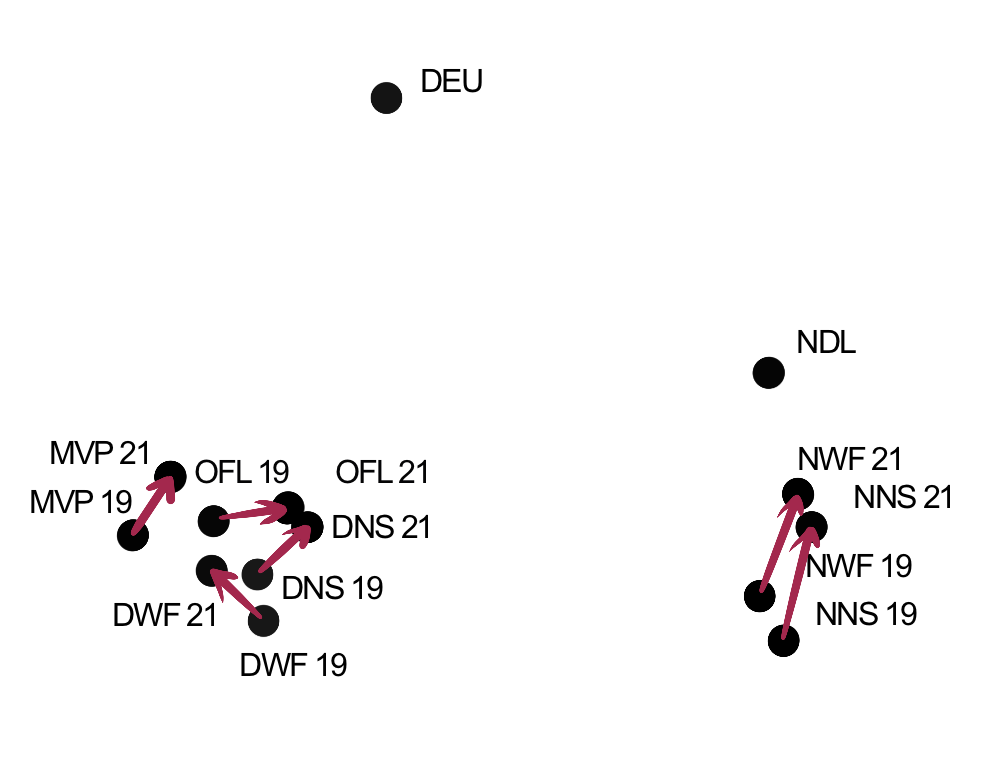
\includegraphics[width=\linewidth]{lut_no-colours_teykenbaseerd_nyde_data_kmeans.png}}
\end{minipage}\hfill%
\begin{minipage}{0.48\textwidth}
    \centering
    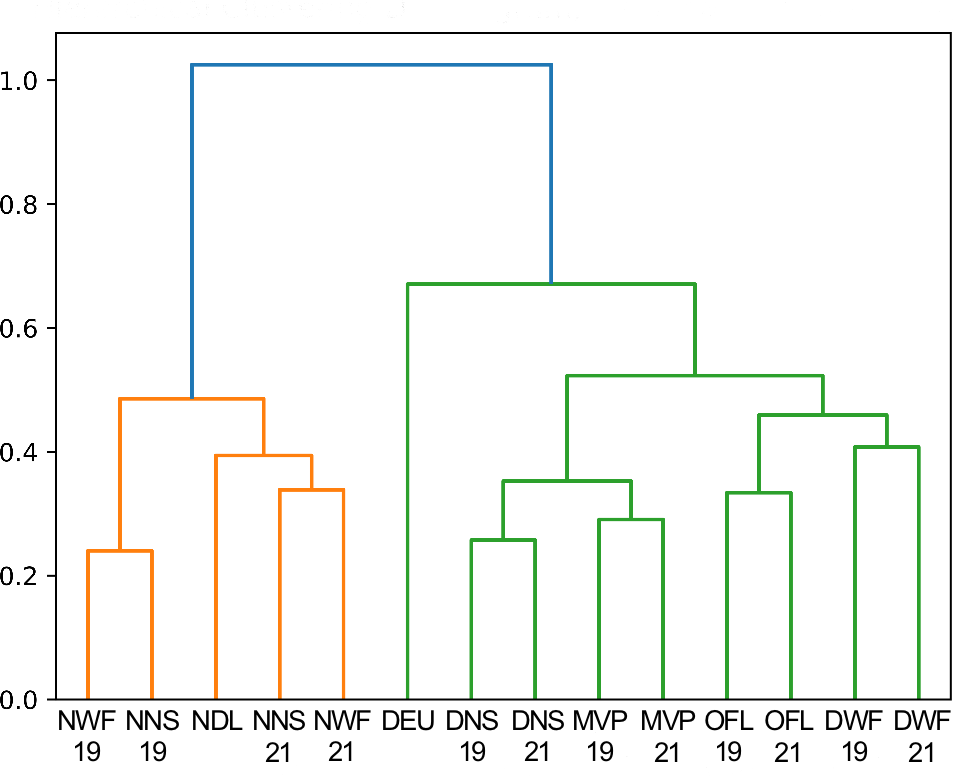
\includegraphics[width=\linewidth]{lut_teykenbaseerd_hierarchical_nyde_data_5levels.png}
    \caption{Character level PCA and hierarchical clustering. (NNS: Dutch North Saxon, NWF: Dutch Westphalian, DNS: German North Saxon, DWF: German Westphalian, MVP: Mecklenburgish--West Pomeranian, OFL: Eastphalian)}
    \label{fig:character_based_clusters}
\end{minipage}%
\end{figure}
The character-based PCA results on the left in \figref{fig:character_based_clusters} show a division into three groups: German Low Saxon (DNS, DWF, MVP, OFL), German (DEU), and Dutch (NDL) with Dutch Low Saxon (NNS, NWF). While the Dutch Low Saxon dialects seem to approach Dutch, German Low Saxon does not show a clear trend of converging towards German. 

On the right, we see a division according to state, likely reflecting different orthographic traditions. Interestingly, the variants from the Netherlands cluster according to century, with older Dutch Low Saxon in one group and late 20\textsuperscript{th} to 21\textsuperscript{st} century Dutch and Dutch Low Saxon in the other. The variants from the German side however, branch according to what we would expect based on the analysis by \citet{Lameli2016}, with a northern (DNS, MVP) and a southern (DWF, OFL) Low Saxon branch that subsequently divide into the major dialect groups. In Dutch Low Saxon, we thus find diachronic differences more strongly pronounced, which can also be seen in the PCA. In German Low Saxon, in contrast, dialectal differences appear more important than diachronic ones. 


\subsection{PoS level}\label{pos-level-results}

\begin{figure}
\begin{minipage}{0.48\textwidth}
    \centering
    \frame{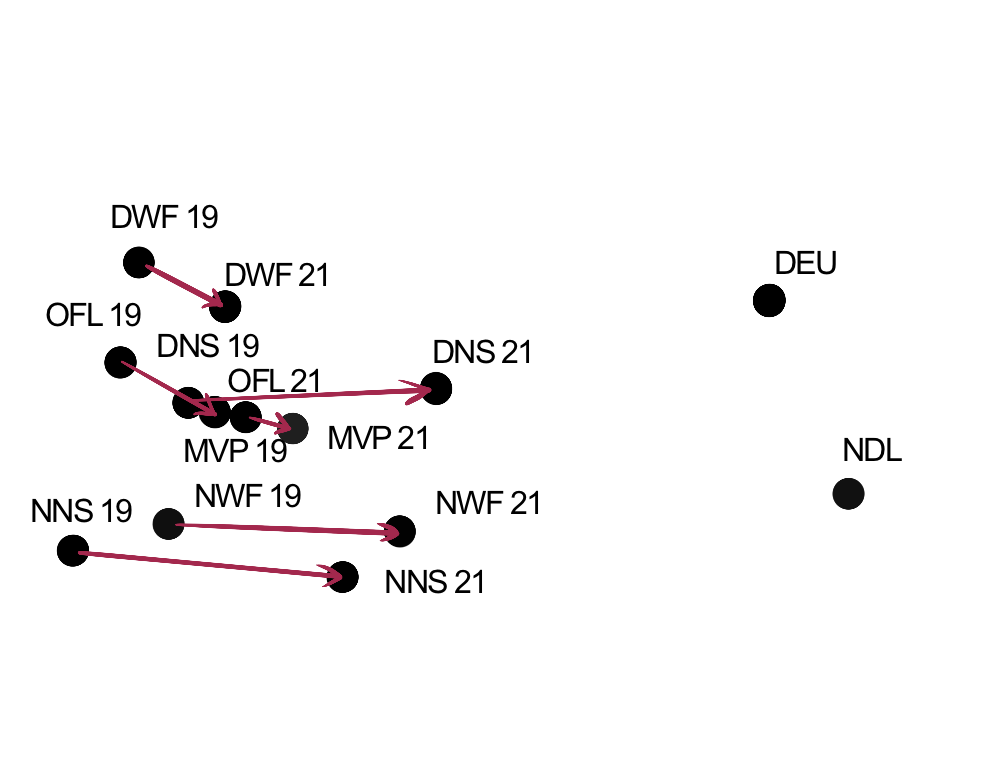
\includegraphics[width=\linewidth]{lut_no-colours_pos_kmeans_3clusters_med_propn.png}}
\end{minipage}\hfill%
\begin{minipage}{0.48\textwidth}
    \centering
    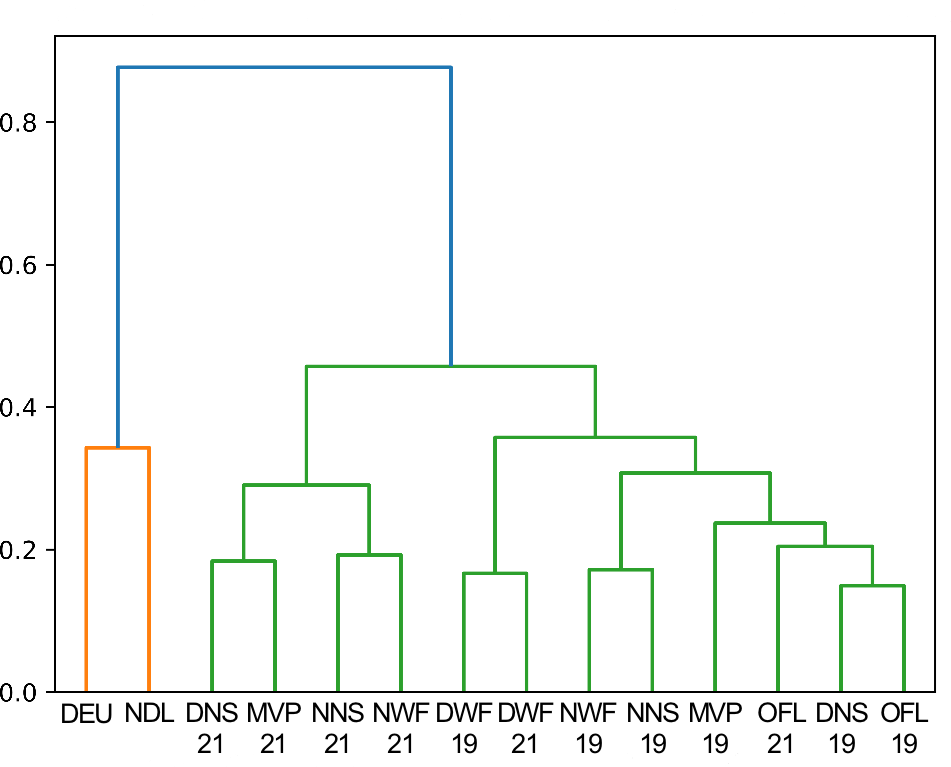
\includegraphics[width=\linewidth]{lut_pos_dendrogram_euclidean_ward_med_propn.png}
    \caption{PoS level PCA and hierarchical clustering.\\NNS: Dutch North Saxon, NWF: Dutch Westphalian, DNS: German North Saxon, DWF: German Westphalian, MVP: Mecklenburgish--West Pomeranian, OFL: Eastphalian}
    \label{fig:pos_based_clusters}
\end{minipage}%
\end{figure}

In \figref{fig:pos_based_clusters}, visualising the PoS results, we see Dutch (NDL) and German (DEU) forming a common group and the Low Saxon dialects forming another one. 
Particularly the PCA results show the Low Saxon dialects approaching the modern state languages Dutch and German. This does, however, not increase the distance along the border in all cases. For example, contemporary German North Saxon (DNS 21) is not placed closer to German Westphalian (DWF) than to the contemporary dialects from the Dutch side (NNS 21, NWF 21). 

In the hierarchical clustering, we find a somewhat corresponding constellation where the contemporary northern branch from Germany (DNS 21, MVP 21) forms a cluster with contemporary Dutch Low Saxon (NNS 21, NWF 21), while the remaining Low Saxon dialects form another cluster. Within this second cluster, we find German Westphalian (DWF) branching off first while older Dutch Low Saxon (NNS 19, NWF 19) is placed closer to Eastphalian (OFL) and the older variants of the northern branch of German Low Saxon (DNS 19, MVP 19). 

In the use or lack of the article described in \sectref{feature:lack-of-definite-article}, we indeed see similar trends to what \citet{Pheiff2022} described. For the n-gram (`\textsc{adp}', `\textsc{det}', `\textsc{noun}'), we find the lowest score in older Dutch North Saxon (NNS 19, NWF 19). However, comparing the older part of the dataset to the contemporary one, we can observe the score to increase for all dialects except Mecklenburgish--West Pomeranian (MVP). Similarly, for the n-gram (`\textsc{adp}', `\textsc{det}', `\textsc{adj}'), all Low Saxon variants -- both older and contemporary -- receive a score lower than Dutch (NDL) and German (DEU), and, again apart from Mecklenburgish--West Pomeranian (MVP), show an increase towards the modern period. Also, the scores for the n-gram (`\textsc{det}', `\textsc{propn}') show lower values for all Low Saxon varieties compared with Dutch (NDL) and German (DEU). Again, an increase can be attested in all varieties except one. A slight decrease can be seen in German North Saxon (DNS).

Dialect differences can also be found for the infinitive construction with \textit{üm}, cf.~\sectref{to-infinitive}, represented by the n-gram (`\textsc{sconj}', `\textsc{part}', `\textsc{verb}').\footnote{Although this does not cover cases with an object or adverb between the \textit{üm} and the \textit{to}, it can still give us a rough idea of the usage.} We do not find this n-gram in the German North Saxon (DNS) or Mecklenburgish--West Pomeranian (MVP) part of the dataset. Neither do we find it in the older Dutch North Saxon (NNS 19, NWF 19) or older Eastphalian (OFL 19), but this could be due to the small amount of data in these two varieties (cf.~\tabref{tab:datasetsize}) and the relative rarity of the construction, as it does appear in the larger contemporary dataset. German Westphalian (DWF) receives comparable scores to German (DEU) (0.00015) in both parts of the dataset (0.00011 and 0.00014). Dutch Westphalian (NWF), on the other hand, shows a decrease from 0.00093 to 0.00015, a score similar to German (DEU) and German Westphalian (DWF).

At the PoS level, we cannot observe a clear tendency of Low Saxon growing apart at the political border. While the increase in article usage brings the dialects closer to Standard Dutch (NDL) and German (DEU), this same development occurs on both sides of the border. Instead, we find a particular closeness of Dutch Low Saxon (NNS, NWF) to the northern dialects (DNS, MVP) in Germany and to a somewhat lesser degree to Eastphalian (OFL).  

\subsection{PoS and morphological features}\label{posmorf-level-results}
%Auch ohne PoS testen, Nur Unigramme? 
%

In \figref{fig:posmorph_based_clusters}, the distance to Dutch (NDL) is disproportionally increased by the gender feature. Since Dutch does not distinguish between masculine and feminine gender in nouns anymore, these receive the tag \texttt{Gender=Fem,Masc}, while Low Saxon and German nouns mostly receive the distinct gender features \texttt{Gender=Fem} or \texttt{Gender=Masc}. Compare \figref{fig:posmorph_based_clusters_without_m-f}, where the \textit{masculine} and \textit{feminine} value of this feature have been replaced by \textit{com} in the whole dataset. This does, however, not seem to obscure the general trends of development within Low Saxon.

\begin{figure}
\begin{minipage}{0.48\textwidth}
    \centering
    \frame{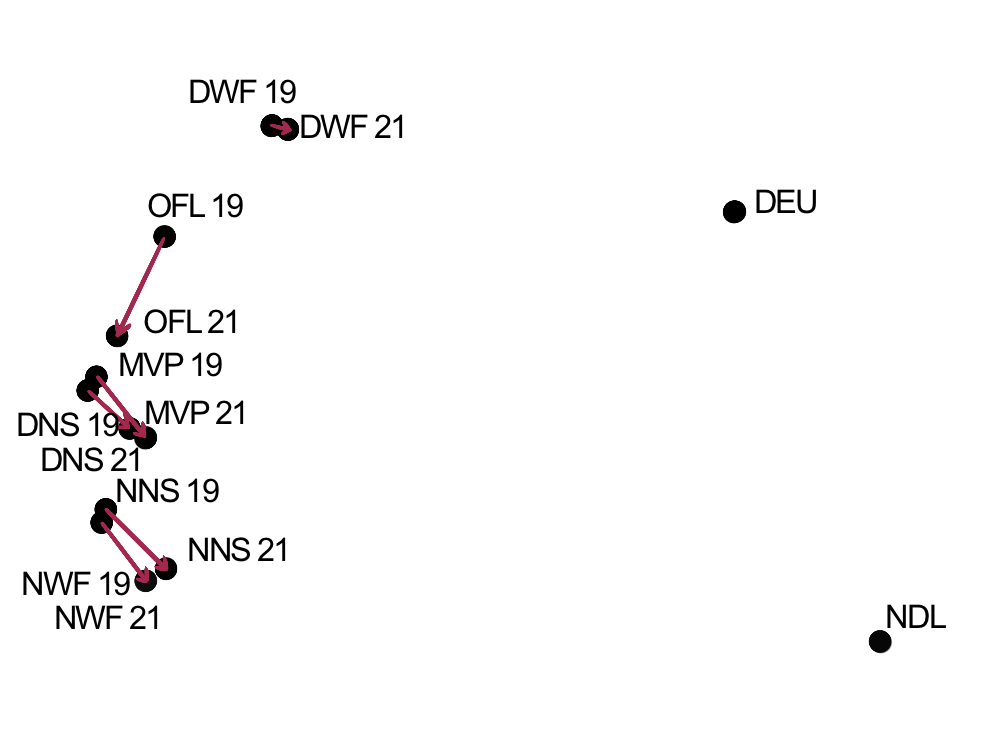
\includegraphics[width=\linewidth]{lut_no-colours_postag-un-morf_kmeans_3clusters_med_propn.png}}
\end{minipage}\hfill%
\begin{minipage}{0.48\textwidth}
    \centering
    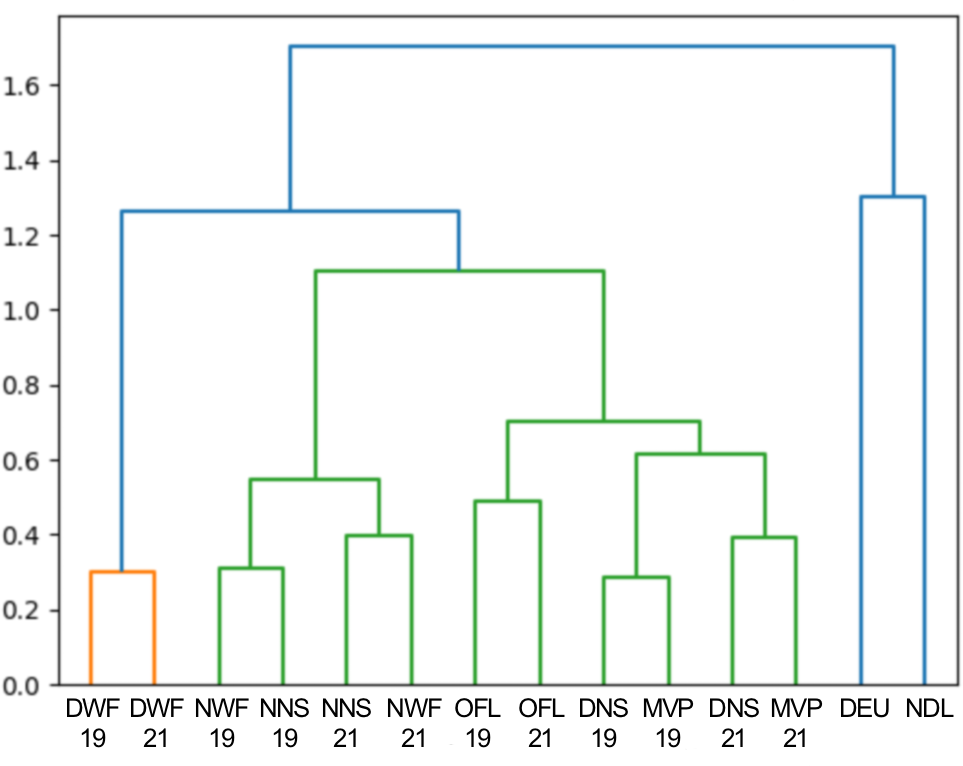
\includegraphics[width=\linewidth]{lut_pos-med-morf_dendrogram_euclidean_ward_med_propn_5levels.png}
    \caption{PoS and morphological features, PCA and hierarchical clustering.\\NNS: Dutch North Saxon, NWF: Dutch Westphalian, DNS: German North Saxon, DWF: German Westphalian, MVP: Mecklenburgish--West Pomeranian, OFL: Eastphalian}
\label{fig:posmorph_based_clusters}
\end{minipage}%
\end{figure}

\begin{figure}
\begin{minipage}{0.48\textwidth}
    \centering
    \frame{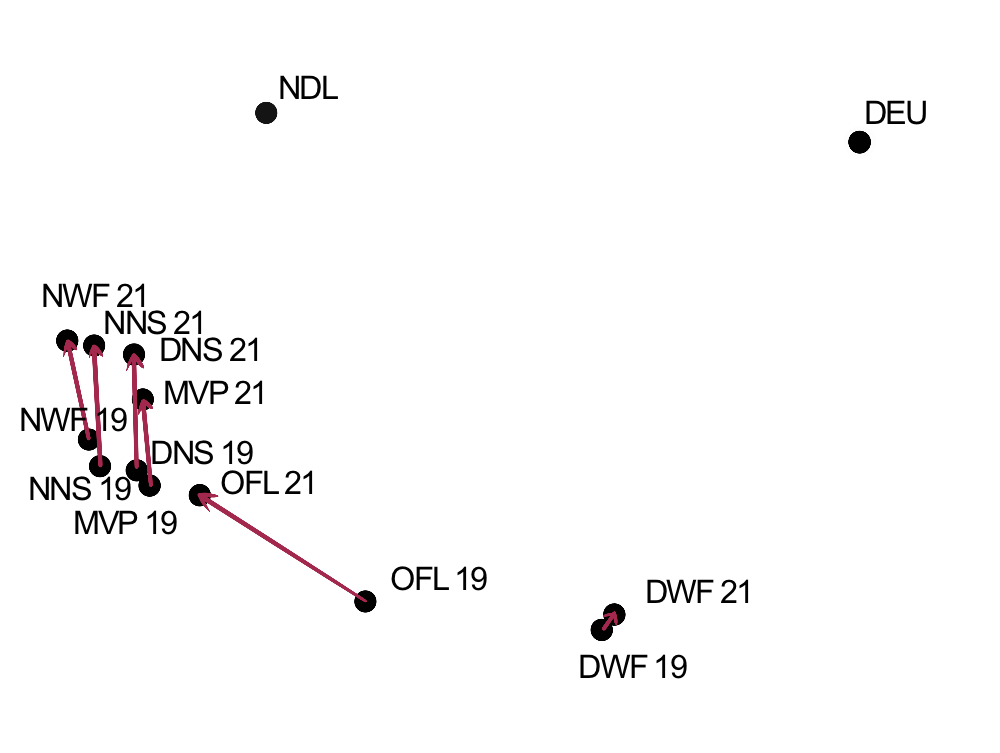
\includegraphics[width=\linewidth]{lut_no-colours_postag-un-morf_kmeans_3clusters_med_propn_gender=com.png}}
\end{minipage}\hfill%
\begin{minipage}{0.48\textwidth}
    \centering
    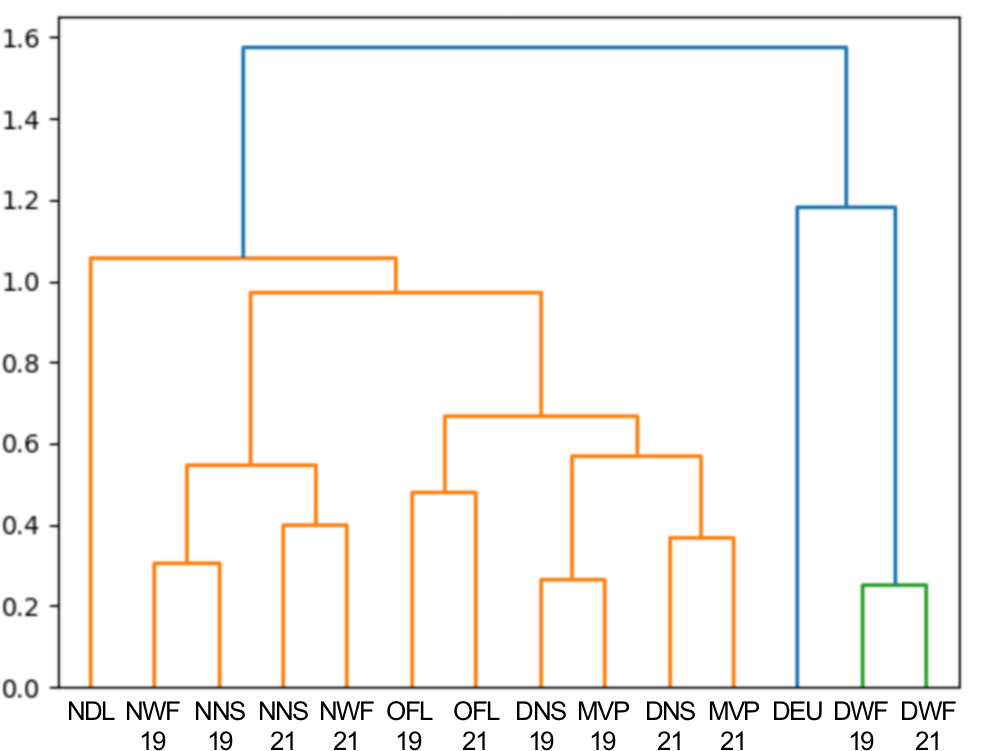
\includegraphics[width=\linewidth]{lut_pos-med-morf_dendrogram_euclidean_ward_med_propn_5levels_gender=com.png}
    \caption{PoS and morphological features, PCA and hierarchical clustering, without feminine--masculine distinction
    \\NNS: Dutch North Saxon, NWF: Dutch Westphalian, DNS: German North Saxon, DWF: German Westphalian, MVP: Mecklenburgish--West Pomeranian, OFL: Eastphalian}
    \label{fig:posmorph_based_clusters_without_m-f}
\end{minipage}%
\end{figure}


An unexpected finding in the PCA is that not only Dutch Low Saxon (NNS, NWF), but also the northern branch of German Low Saxon (DNS, MVP) converges towards Dutch (NDL). Eastphalian (OFL) on the other hand, appears to approach the northern dialects. In the hierarchical clustering, similar to \figref{fig:pos_based_clusters}, Dutch Low Saxon forms a cluster with Eastphalian and northern German Low Saxon. 

We find German Westphalian (DWF) in an outlier position both in the PCA and in the hierarchical clustering. In \figref{fig:posmorph_based_clusters_without_m-f}, it can even be seen to cluster with German (DEU) instead of the other Low Saxon dialects. In addition to the greater closeness to German, the amount of change in German Westphalian is also strikingly small. Preservation of the dative case, cf.~\sectref{feature:case}, is certainly one feature that contributes to the relative closeness to German. Among the n-grams with the highest scores for both German and German Westphalian, there are several ones containing the \texttt{Case=Dat} feature. 

The subjunctive mood described in \sectref{feature:subjunctive} was unfortunately not learnt properly by the tagger due to its apparent rarity in the training data. As subjunctive forms were tagged as indicative or ambiguous, we cannot draw any conclusions based on our dataset regarding this aspect. 

The IPP construction\footnote{Represented by the bigrams \texttt{('AUX', 'VerbForm=Inf'), ('VERB', 'VerbForm=Inf')} and \texttt{('VERB', 'VerbForm=Inf'), ('AUX', 'VerbForm=Inf')}.} or lack thereof \footnote{Represented by \texttt{('VERB', 'VerbForm=Inf'), ('AUX', 'Tense=Past|VerbForm=Part').}} described in \sectref{IPP} is not among the highest scoring features, as only the bigram
\begin{lstlisting}
('AUX', 'VerbForm=Inf'), ('VERB', 'VerbForm=Inf')
\end{lstlisting}
makes it into the top 500 features for older Dutch Westphalian (NWF) and Dutch (NDL), whereas in most cases, the relevant n-grams are not even among the top 1,000 features. Nonetheless, we do observe dialectal differences, as well as language change here. These, however, only partly reflect the description in the literature. The main finding is that the IPP construction, either with \textit{VERB -- AUX} or with \textit{AUX -- VERB} order, occurs in all Low Saxon dialects and is the preferred construction in most of them. Curiously, it is by far the preferred construction even in both periods of Dutch North Saxon (NNS), while \citet{BloemhoffEtAl2019} claim to not know of the phenomenon. The only varieties showing a clear preference for the non-IPP version, are German North Saxon (DNS) and Mecklenburgish--West Pomeranian (MVP) from the older period.
In the contemporary data, despite the non-IPP construction still occurring frequently, its IPP alternative has started to dominate. This confirms our personal observation that the IPP variant is indeed used as well by Low Saxon speakers today. 

Despite such individual opposing trends, however, none of the German Low Saxon dialects seem to as a whole increasingly resemble German (DEU), and the distance between Dutch Low Saxon (NNS, NWF) and the northern dialects from Germany (DNS, MVP) remains roughly the same. 

\section{Discussion}\label{discussion}

As expected, the three levels under investigation lead to rather different results, in terms of both clustering and observable changes in similarity.  

We assume the character level to largely reflect spelling differences (cf.~\sectref{orthography}) and these are likely behind the noticeable divide between Dutch Low Saxon and German Low Saxon which we do not see in the other experiments. Nevertheless, among the n-grams with the highest tf-idf values, we also find a few that indicate phonological and morphological differences. For instance, we find that the Low Saxon dialects with preserved word-final \textit{e} (DWF, NWF, OFL) receive a higher score for the n-gram (`e', ` ') than the dialects with \textit{e}-apocope in nouns and verbs (DNS, NNS, MVP). Similarly, the highest score for the n-gram (`t',~` ') is found in contemporary German North Saxon (DNS), which uses \textit{-(e)t} as the plural suffix of present tense verbs, while older Mecklenburgish--West Pomeranian (MVP), which typically uses \textit{-(e)n} for the same function, receives the lowest score.

The similarity at the character level is likely distorted by the different orthographic traditions in other ways as well. It could for example be the case that the spellings commonly used for Dutch Low Saxon today make it appear disproportionally Dutch compared with the older variants. This would explain the noticeable shift towards Dutch in the PCA as well as the grouping of contemporary Dutch Low Saxon with Dutch in the hierarchical clustering. Dutch Low Saxon clustering according to time period instead of dialect should however not primarily be attributed to orthography, as we see the same phenomenon at the level of PoS and morphological features as well. 

\begin{sloppypar}
One might have expected a comparable closeness between German Low Saxon and German due to the German-based writing traditions. In addition to morphological differences, an explanation might be found in the High-German consonant shift leading to a different distribution and frequency of many phonemes. The overall clustering within German Low Saxon corresponds well to the findings of \citet{Lameli2016}, and we see a northern group consisting of German North Saxon (DNS) and Mecklenburgish--West Pomeranian (MVP), and a southern group consisting of Westphalian (DWF) and Eastphalian (OFL).
\end{sloppypar}

Despite the common naming, Dutch Westphalian (NWF) could not be shown to be particularly close to German Westphalian (DWF) at any of the levels investigated. Furthermore, the similarity between Dutch North Saxon (NNS) and Dutch Westphalian (NWF) appears to be roughly equal to the similarity between German North Saxon (DNS) and Mecklenburgish--West Pomeranian (MVP). This supports the idea that if, in line with \citet{Lameli2016}, the north-western part of German Westphalian shares more features with the northern dialects than with the other Westphalian varieties, the neighbouring varieties on the Dutch side of the border might also share more traits with northern Low Saxon. 

The two lines we mainly wanted to investigate -- the Dutch-German border and the traditional East-West division in German Low Saxon -- did not present themselves as clearly as we had expected. 

An East-West division could not be found at any of the levels under scrutiny. On the contrary, German North Saxon (DNS) and Mecklenburgish--West Pomeranian (MVP) actually appear so close that they cluster according to century instead of dialect at both the PoS and the morphological level. It would be desirable to repeat these experiments with additional eastern dialects when more data becomes available. 

A certain distance between Dutch Low Saxon (NNS, NWF) and the northern dialects from Germany (DNS, MVP) is observable and might be attributed to influence from the different state languages. The distance is however not bigger than between the northern German Low Saxon dialects and German Westphalian (DWF). In particular, the border does not explain why the northern dialects from Germany would converge towards Dutch (NDL) instead of German (DEU). Thus, the situation appears to be more complex.  

On the one hand, the loss of morphological complexity, especially the loss of case inflection, could be one factor behind the increasing similarity between Dutch (NDL) and northern German Low Saxon (DNS, MVP).
Another factor that should be taken into consideration is the ongoing strife to codify Low Saxon, in particular in Germany, where textbooks and grammar descriptions for school and adult education have been published in several dialects.

Due to this available documentation, the people who produce written German Low Saxon are probably very aware of the differences between Low Saxon and German. Moreover, they presumably strive to produce what they consider “good Low Saxon”, which is not necessarily the same form of language they would informally speak at home with family and friends but might be an idealised form of their dialect where features distinct from German are preferred. 

Furthermore, thanks to the internet and social media in particular, it has become easier to access content in other dialects and from the other side of the border. We are aware that several people who provided data have interdialectal and some even cross-border contact. 

As a result from the larger number of speakers, northern German Low Saxon (DNS, MVP) is better represented in media and literature, which could explain why Eastphalian (OFL) appears to be converging towards the northern dialects.  

Language skills might play a role as well, as the respective state language is not necessarily the only additional language of which Low Saxon writers have knowledge. 
Some of the people from whom we received texts are to different degrees proficient in the other state language or in Scandinavian languages as well. Especially in case of younger speakers, knowledge of English can be assumed and English influence on the Low Saxon of younger second language or heritage learners might be a topic worth investigating. 

%Eastphalian approaching the northern dialects due to stronger representation in media and literature? 

%Since this (LS not growing apart but even seemingly slightly approaching each other) appears rather counterintuitive at first, listeners will probably expect explanations. Below some possibly relevant factors that come to mind:

%- There has been a striving to codify LS, in Germany even more so than in the Netherlands. For many LS dialects in Germany, there are dictionaries, textbooks and grammar descriptions.
%- There is less material in the Netherlands and it does seem less aimed at guiding people's production or systematically teaching the language to non-speakers, maybe more for understanding and as lists of curious characteristics or words. E.g,  dictionaries generally don't contain information on gender or inflection.
%- I would assume that - probably at least partly thanks to the available documentation - people who produce written GLS today are quite aware of the differences between German and LS. They might be language activists themselves and probably strive to produce what they consider good LS - which is not necessarily the same form of language they would informally speak at home with family or friends, but might be an idealised form of their dialect.
%- Thanks to the internet and social media in particular, it has become a lot easier to consume content in other dialects and even get in contact with LS speakers from the other side of the border.
%- Of at least some of the people who provided modern data from Germany, I know that they have interdialectal, some even cross-border contacts. At least one of them has studied Dutch. Some speak Scandinavian languages.
%- In particular in younger generations, the local majority language is not the only contact language for LS. Virtually everyone is regularly exposed to English, many speak or have at least studied additional languages.

\section{Limitations and future research}

We have so far based our comparisons of Low Saxon dialect similarity only on PCA and hierarchical clustering. We can therefore not preclude that other clustering approaches or a different implementation of the same clustering methods might yield different results. Furthermore, we would like to test a greater variety of visualisation techniques. For instance, a map format might be easier to grasp, especially for readers less familiar with the Low Saxon language area.

Another factor of uncertainty is the automatic tagging that our work relies on. 
Upon manual inspection of the n-grams, we have become aware of issues with the tagging of certain features. One of these is the gender feature. Even in the dialects that have preserved a three-fold distinction, the form of a possible accompanying article or adjective does not necessarily fully disambiguate the gender of the noun. This poses a challenge for both the automatic tagger and for the human annotator as the gender of nouns can differ from dialect to dialect and might not be documented for the precise dialect in question. 
In particular, the Dutch Low Saxon dialects in the process of losing their feminine-masculine distinction pose problems as it is not always obvious when a gender distinction can still be assumed. 



The unfortunate fact that our tagger did not learn to recognise the subjunctive has shown that rare features can require careful manual selection of the training data. In the German and Low Saxon sentences randomly selected for manual annotation and subsequent fine-tuning, this feature apparently did not occur frequently enough. 

Another tagging-related risk concerns the finetuning to different groups of dialects. Since the finetuning sets consist of only around 200 to 300 sentences per group, some overfitting to a particular subset of the data might have happened. Nevertheless, we considered the finetuning justified due to the substantial spelling variation described in \sectref{orthography}. There are, for instance, several cases of character strings that would receive different PoS tags in different dialects: For instance, \textit{doe} as the personal pronoun of the second person singular in Gronings (part of NNS) receives the tag `\textsc{pron}'; as the definite article in East Westphalian (part of DWF) it is tagged as `\textsc{det}' and, in addition, it is a possible spelling for the 1\textsuperscript{st} person singular present tense of the verb \textit{doon} `to do' in, e.g., German North Saxon (DNS) and Dutch Westphalian (NWF), when it should be tagged as `\textsc{verb}' or possibly `\textsc{aux}'. Neither can we rule out that this finetuning might cause the varieties within the same group to appear closer than they are. While the members of the same group do at least not appear artificially close, compare, for instance, the German South Low Saxon group consisting of Eastphalian (OFL) and German Westphalian (DWF) in Figures~\ref{fig:posmorph_based_clusters} and \ref{fig:posmorph_based_clusters_without_m-f} or the two periods of Dutch Low Saxon: Dutch North Saxon (NNS) and Dutch Westphalian (NWF) in \figref{fig:pos_based_clusters}, larger and more diverse finetuning sets would certainly be desirable. 

The different size of the dialect regions should not be neglected either. The German Low Saxon regions are noticeably larger than the Dutch Low Saxon ones, and most of the German Low Saxon texts in our dataset are not from areas particularly close to the border. Several of the German North Saxon (DNS) writers come from Schleswig-Holstein or Hamburg, while in the German Westphalian dataset (DWF), East Westphalian and South Westphalian are overrepresented. Varieties from border regions, such as East Frisian and West Munsterlandic, might have exhibited greater similarity with Dutch Low Saxon. 

The lack of diversity among the writers is a problem in some dialects as well, in particular in contemporary German Westphalian (DWF) and Eastphalian (OFL), and in older Mecklenburgish--West Pomeranian (MVP). Contemporary Eastphalian is unfortunately only represented by one writer so far, which is why some of the developments we observe might simply be features of this writer's idiolect. While in contemporary German Westphalian, we have obtained texts from a variety of writers, these mostly represent the older generation born in the first half of the 20\textsuperscript{th} century. Even though the texts themselves were published in the late 20\textsuperscript{th} or the 21\textsuperscript{st} century, their language might be more representative of the older period. This would explain why we see so little change in German Westphalian both at the PoS and the morphological level. 
The older Mecklenburgish--West Pomeranian part of the dataset also includes texts from a variety of sources but works by Fritz Reuter clearly dominate. The fact that the older part of the Mecklenburgish--West Pomeranian data scores higher in article use than the newer part, could thus possibly result from characteristics of Reuter's idiolect.
The collection of additional data for these dialects would therefore be desirable.

An additional desideratum is the comparison with Dutch and German from the 19\textsuperscript{th} -- early 20\textsuperscript{th} century. While the convergence towards the state languages that we see at the PoS level seems intuitive, we cannot yet rule out the possibility that all three languages develop into a similar direction.

Some structures such as the double complementiser with \textit{as/dat} described in \sectref{feature:double-complementiser} that we initially planned to  include, turned out to require lemma information since the PoS bigram \textit{ADV -- SCONJ} representing, e.g., \textit{worüm dat} `why', captures several unrelated constructions as well. We are already working on automatic lemmatisation for Low Saxon and are planning to study lexical differences as well in our future work. 


%Compute the features that show the biggest change, something to do for the final version? 

\section*{Abbreviations}
\begin{tabular}{@{}llll@{}}
MMM & German                         & NDL & Dutch\\
DEU & German                         & NNS & Dutch North Saxon\\
DNS & German North Saxon             & NWF & Dutch Westphalian\\
DWF & German Westphalian             & OFL & Eastphalian \\
MVP & Mecklenburgish-West Pomeranian & PoS & Part of Speech\\
\end{tabular}
\section*{Acknowledgements}

\begin{sloppypar}
We would like to thank Kevin Behrens, Behrend Böckmann, Johanna Bojarra, Marita Bojarra, Christiane Ehlers, Marianne Ehlers, Heiko Gauert, Jan Graf, Bernd Lubs, Christian Peplow, Karl Peplow, Gennadi Ratson, Heinrich Siefert and Florian Wille for providing additional texts in the northern dialects from Germany! 
\end{sloppypar}

This work has been supported by the Academy of Finland through project No.~342859 ``CorCoDial -- Corpus-based computational dialectology''.

\printbibliography[heading=subbibliography,notkeyword=this]
\end{document}

%\appendix

%\section{Morphology without feminine -- masculine distinction}\label{without_m-f}
% % % % 
% % % % \begin{table}
% % % % \caption{Frequencies of word classes}
% % % % \label{tab:myname:frequencies}
% % % %  \begin{tabularx}{.8\textwidth}{X rrrr}
% % % %   \lsptoprule
% % % %             & nouns & verbs  & adjectives & adverbs\\
% % % %   \midrule
% % % %   absolute  &   12  &    34  &    23      & 13\\
% % % %   relative  &   3.1 &   8.9  &    5.7     & 3.2\\
% % % %   \lspbottomrule
% % % %  \end{tabularx}
% % % % \end{table}
% % % % 
% % % % 
% % % % 
% % % % \is{Cognition} %add "Cogntion" to subject index for this page
% % % % 
% % % % \ea
% % % % \gll cogito                           ergo      sum\\
% % % %      think.\textsc{1sg}.\textsc{pres} therefore \textsc{cop}.\textsc{1sg}.\textsc{pres}\\
% % % % \glt `I think therefore I am.'
% % % % \z
% % % % \il{Latin} %add "Latin" to language index for this page
